\documentclass[11pt,a4paper]{article}

\usepackage[margin=2.5cm]{geometry}
\usepackage[T1]{fontenc}
\usepackage[utf8]{inputenc}
\usepackage{lmodern}
\usepackage{microtype}
\usepackage{graphicx}
\usepackage{booktabs}
\usepackage{array}
\usepackage{amsmath}
\usepackage{amssymb}
\usepackage{algorithm}
\usepackage{algpseudocode}
\usepackage{hyperref}
\usepackage{cleveref}
\usepackage{enumitem}
\usepackage{caption}
\usepackage{subcaption}
\usepackage{xcolor}
\usepackage{tikz}
\usetikzlibrary{arrows.meta,positioning}
\usepackage[none]{hyphenat}

\hypersetup{
    colorlinks=true,
    linkcolor=blue!50!black,
    citecolor=blue!50!black,
    urlcolor=blue!50!black
}

\graphicspath{{figures/}{image/}}
\setlength{\parskip}{0.3cm}
\setlength{\parindent}{0pt}
\sloppy

\makeatletter
\providecommand{\theHALG@line}{\thealgorithm.\arabic{ALG@line}}
\makeatother

\newcolumntype{L}[1]{>{\raggedright\arraybackslash}p{#1}}
\newcommand{\blueprintimage}[1]{%
    \IfFileExists{image/#1}{%
        \includegraphics[width=\linewidth,height=0.40\textheight,keepaspectratio]{#1}%
    }{%
        \fbox{\parbox[c][0.13\textheight][c]{0.92\linewidth}{\centering Image placeholder\\\ttfamily\detokenize{#1}}}%
    }%
}
\tikzset{
    prodraw/.style={draw, rounded corners=2pt, align=center, font=\scriptsize, minimum width=2.7cm, minimum height=0.95cm, text width=2.45cm},
    rawnode/.style={prodraw, fill=gray!10},
    machinenode/.style={prodraw, fill=blue!6},
    finalnode/.style={prodraw, fill=green!8},
    prodarrow/.style={-Latex, thick},
    edgelabel/.style={font=\tiny, fill=white, inner sep=1pt, midway, above=2pt}
}

\title{AutoBlueprint: Autonomous Agent Design for Compact Factory Blueprint Generation}
\author{Zecheng Tang 20513308\\ COMP3004 Designing Intelligent Agents}
\date{May 2026}

\begin{document}

\maketitle

\begin{center}
    \begin{minipage}{0.48\linewidth}
        \centering
        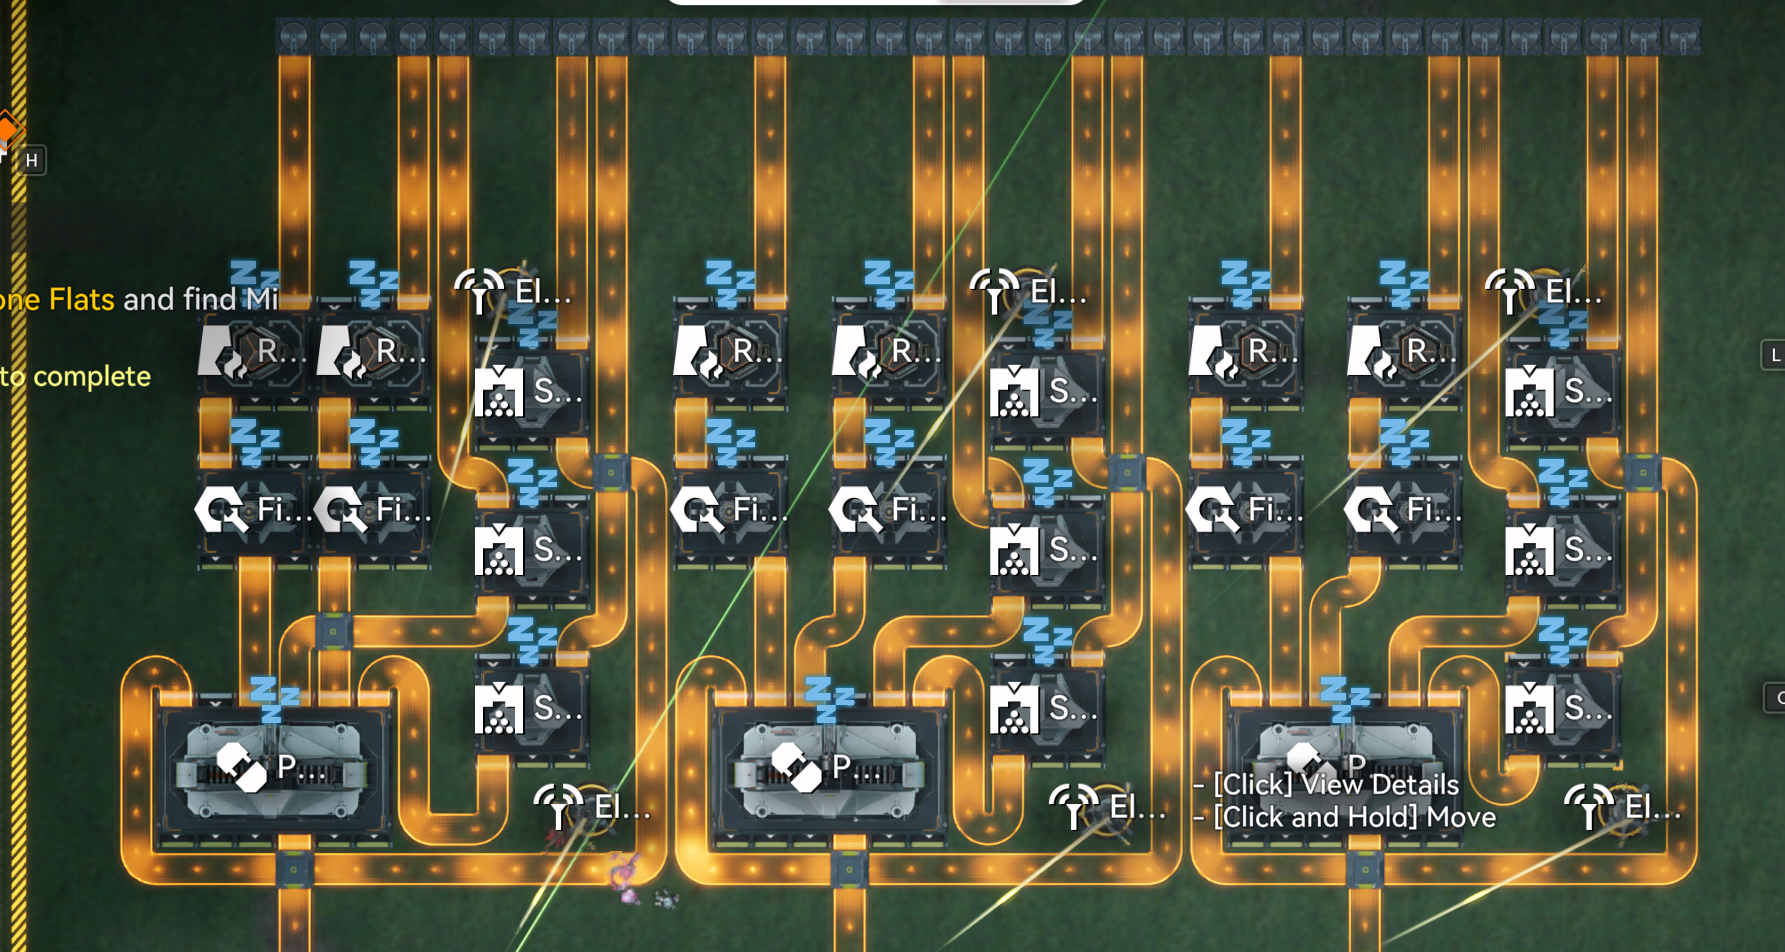
\includegraphics[width=\linewidth,height=0.22\textheight,keepaspectratio]{Actual_High.png}
        \captionof*{figure}{Actual blueprint}
    \end{minipage}\hfill
    \begin{minipage}{0.48\linewidth}
        \centering
        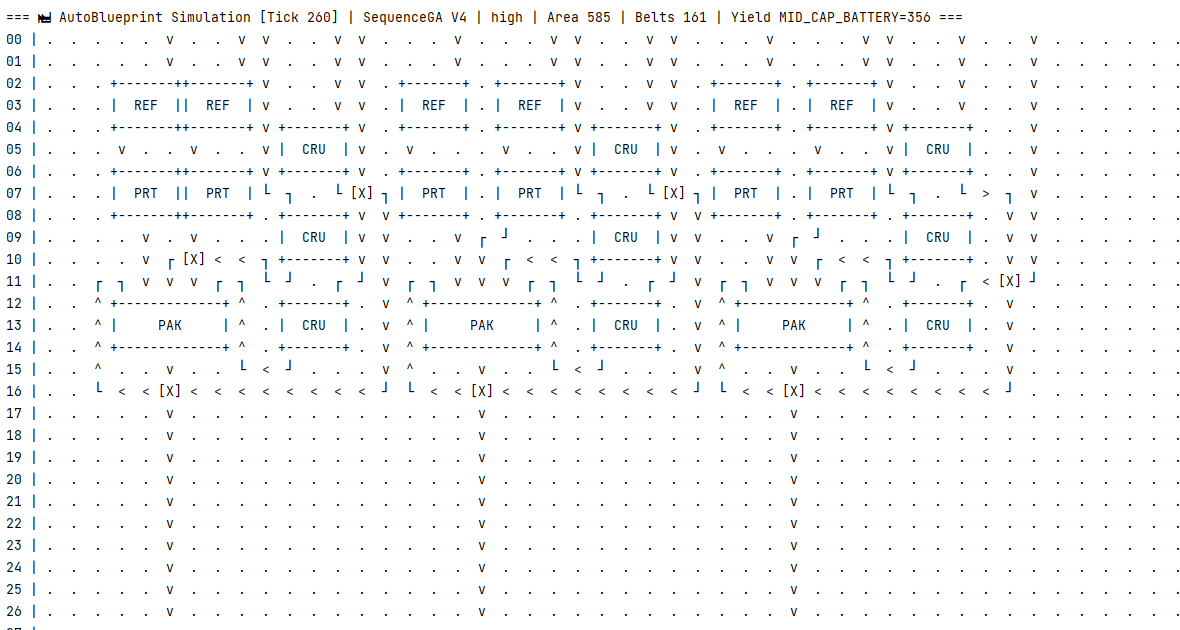
\includegraphics[width=\linewidth,height=0.22\textheight,keepaspectratio]{SequenceGA_High.png}
        \captionof*{figure}{SequenceGA output}
    \end{minipage}
\end{center}


\clearpage
\tableofcontents
\clearpage



\begin{abstract}
AutoBlueprint is an autonomous agent system for generating compact and physically valid factory blueprints. The environment models machines, recipes, ports, transport belts, and grid constraints. The project compares a rule-based baseline with search and optimisation agents using best area, best belt length, routing success, and successful production of the required output amount.
\end{abstract}

\section{Introduction}
\label{sec:introduction}

Factory automation games and production simulators pose a useful model problem for intelligent agents: a designer must transform a target product and rate into a valid arrangement of machines and transport components. This requires reasoning about recipes, throughput, space, ports, and routing.

AutoBlueprint addresses this problem by treating blueprint generation as an autonomous agent task. Given a target product, the agent perceives a symbolic production environment, decides which machines and transport components are required, places them on a grid, and attempts to connect the resulting material flows.

\subsection{Research question}
How do different autonomous blueprint-generation agents compare in producing compact, valid, and routable factory layouts under the same production requirements?

\subsection{Contributions}
\begin{itemize}[leftmargin=*]
    \item A grid-based factory environment with explicit machines, materials, ports, recipes, and transport components.
    \item Several autonomous agents for blueprint generation, including a rule-based baseline and optimisation-based variants.
    \item An experimental comparison using measurable layout and routing metrics.
\end{itemize}

\section{Background and Related Work}
\label{sec:background}

\subsection{Agents, Layout, and Search}

An autonomous agent perceives an environment and selects actions to achieve a task \cite{russell2021ai}. In AutoBlueprint, percepts are recipes, machine properties, ports, and grid occupancy; actions are instantiation, placement, orientation, and routing. Since one placement can block later belts, the task requires deliberation.

Factory layout generation is related to facility layout, where machines are arranged under spatial constraints while reducing material-handling cost \cite{drira2007facility}. AutoBlueprint is smaller and game-oriented, but keeps the same trade-off between compactness, flow efficiency, and access space. Sequence-pair representations from rectangle packing and VLSI placement \cite{murata1996rectangle} are relevant because the buildings are rectangular modules with relative ordering constraints.

\subsection{Routing and Optimisation}

Routing is graph search over grid cells, with buildings and existing transport as obstacles. A* combines path cost with a distance heuristic \cite{hart1968astar}. For placement, simulated annealing explores large spaces by sometimes accepting worse moves early \cite{kirkpatrick1983annealing}. AutoBlueprint combines recipe reasoning, placement search, and routing validation.

\section{System Overview}
\label{sec:system}

AutoBlueprint is a controlled production-layout environment. Given a target product and rate, an agent produces a grid blueprint with machines, transport, and directed material flows. Recipes define the production graph; the grid tests whether it can be placed and routed under size, port, collision, and compactness constraints.

\subsection{Environment Model}

The \texttt{GridMap} class represents a fixed-size two-dimensional grid. Cells may be empty, occupied by a building, or occupied by transport. The environment checks boundaries, collisions, rotation-dependent size, bridge endpoints, and active ports. Tick updates move items through buildings and transport, so blueprints are tested as working layouts rather than static drawings.

\subsection{Entity and Recipe Representation}

The environment is built from materials, buildings, and transport components. \Cref{tab:entity-attributes} lists the attributes used for production and feasibility reasoning.

\begin{table}[H]
    \centering
    \caption{Core attributes of the main entity types.}
    \label{tab:entity-attributes}
    \begin{tabular}{L{0.20\linewidth} L{0.40\linewidth} L{0.30\linewidth}}
        \toprule
        Entity type & Main attributes & Purpose in the system \\
        \midrule
        Material &
        Material Type; Material State, either solid or liquid. &
        Defines produced or transported items and whether belts or pipes are legal. \\
        \addlinespace
        Building &
        Component ID; Name; Size; System Type; Input Materials; Output Materials; Production Speed; Inventory Capacity; Power Fields; Direction; Input Side; Output Side; Active Input Ports; Active Output Ports; Direct Insertion Flag; Omni Port Flag. &
        Defines footprint, recipe behaviour, throughput, ports, and direct insertion. \\
        \addlinespace
        Transport component &
        Component ID; Name; Position; Direction; Current Item; Next Tick Item; Maximum Capacity; System Type; Supported Material State; Optional Bridge End Position; Component Specific Routing Logic. &
        Moves material through straight belts, splitters, mergers, crossers, access parts, and bridges. \\
        \bottomrule
    \end{tabular}
\end{table}

Materials distinguish solid and liquid items. Buildings store recipes and ports. Transport components form the logistics network, and \texttt{registry} returns fresh catalogue objects so inventories and buffers are not shared.

\subsection{Two Logistics Systems}

System A follows \textit{Mindustry}, a factory-management and tower-defense game with conveyor logistics \cite{mindustrywikipedia,mindustrywiki}. It uses omni-directional ports and may allow direct insertion. System B follows \textit{Arknights: Endfield}, whose industrial systems include automated chains and conveyor routing \cite{endfieldwikipedia,endfieldwiki}. Its buildings have directional ports and require access parts, belts, pipes, splitters, mergers, or crossers.

All evaluated agents use System B because its explicit transport-space requirement better exposes planning ability.

\subsection{Task Definition}

The agent must infer the production chain, instantiate machines, place and orient them, and connect material flows. A valid blueprint stays inside the map, avoids overlap, respects material state and port rules, and can produce the target. The objective is validity, compactness, and routability.

\subsection{Agent-Environment Interaction}

The interaction follows a perceive-plan-act-evaluate cycle: read the catalogue and target, build a production graph, place and route entities, then evaluate area, belt length, routing, and production.

\begin{figure}[H]
    \centering
    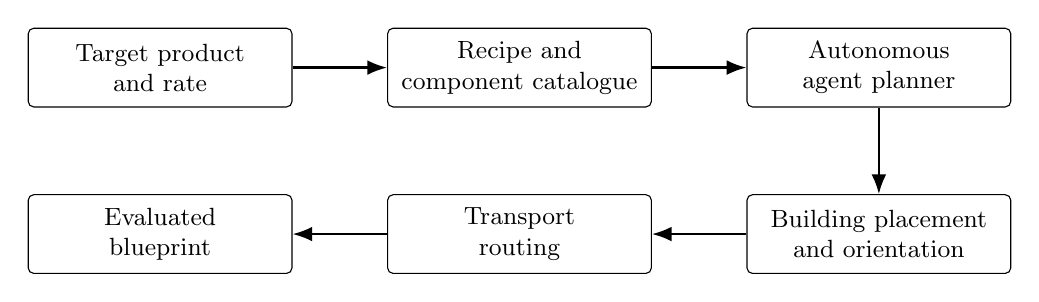
\begin{tikzpicture}[
        node distance=1.1cm and 1.2cm,
        flowstep/.style={
            draw,
            rounded corners=2pt,
            align=center,
            minimum width=3.35cm,
            minimum height=1.0cm,
            font=\small
        },
        arrow/.style={-{Latex[length=2.5mm]}, thick}
    ]
        \node[flowstep] (target) {Target product\\and rate};
        \node[flowstep, right=of target] (catalogue) {Recipe and\\component catalogue};
        \node[flowstep, right=of catalogue] (planner) {Autonomous\\agent planner};
        \node[flowstep, below=of planner] (placement) {Building placement\\and orientation};
        \node[flowstep, left=of placement] (routing) {Transport\\routing};
        \node[flowstep, left=of routing] (evaluation) {Evaluated\\blueprint};

        \draw[arrow] (target) -- (catalogue);
        \draw[arrow] (catalogue) -- (planner);
        \draw[arrow] (planner) -- (placement);
        \draw[arrow] (placement) -- (routing);
        \draw[arrow] (routing) -- (evaluation);
    \end{tikzpicture}
    \caption{High-level AutoBlueprint system flow. The agent transforms a symbolic production requirement into a physical grid blueprint and receives feedback through validity and quality metrics.}
    \label{fig:architecture}
\end{figure}

\section{Agent Design}
\label{sec:agent-design}

All agents transform a symbolic target into a physical System B blueprint. The versions are iterative: each keeps useful earlier mechanisms while addressing area, routing, blocked ports, congestion, or instability.

\subsection{Shared Pipeline and Production Graph}

Most agents build a production graph, search for positions and directions, commit the layout, and route each logical edge. Later agents feed routing information back into layout search because compact placement is useful only when transport can also be placed legally.

The production graph is generated backwards from the target. Raw inputs terminate expansion; other materials require a recipe, producer instances, and upstream demands. Early agents use round robin matching, while later versions add capacity quotas or min cost flow.

\begin{algorithm}[H]
    \caption{Backward production graph construction}
    \label{alg:production-graph}
    \begin{algorithmic}[1]
        \State Initialise demand queue with the target output requirements
        \While{demand queue is not empty}
            \State Pop material $m$ and required amount $a$
            \If{$m$ is an available raw input}
                \State Mark $m$ as an external input
            \Else
                \State Find recipe $r$ and producer building for $m$
                \State Instantiate $\lceil a / \mathrm{rate}(r,m)\rceil$ producer buildings
                \State Add scaled input demands of $r$ to the queue
            \EndIf
        \EndWhile
        \State Match producer instances to consumer instances using the family specific rule
        \State \Return directed production graph
    \end{algorithmic}
\end{algorithm}

\subsection{Agent Families and Version Evolution}

The families progress from deterministic placement to routing-aware optimisation and richer layout representations.

\begin{table}[H]
    \centering
    \caption{Agent versions and algorithmic ideas.}
    \label{tab:agent-versions}
    \begin{tabular}{L{0.30\linewidth} L{0.60\linewidth}}
        \toprule
        Agent version & Algorithm / logic \\
        \midrule
        \texttt{GenericBaselineAgent} &
        Rule-based block layout with A* routing. \\
        \addlinespace
        \texttt{SABaselineAgent} / SA V1 &
        Coordinate-based simulated annealing. \\
        \addlinespace
        \texttt{SAAgentV2} &
        Routing-aware simulated annealing with failure feedback. \\
        \addlinespace
        \texttt{FdpSaAgent} V1 &
        Force-directed placement followed by SA refinement. \\
        \addlinespace
        \texttt{FdpSaAgentV2} &
        Multi-start routing-aware FDP+SA. \\
        \addlinespace
        SequenceSA V1 (\texttt{SequencePairSaAgentV1}) &
        Sequence-pair module floorplanning. \\
        \addlinespace
        SequenceSA V2 (\texttt{SequencePairSaAgentV2}) &
        Production-cell B*-tree packing. \\
        \addlinespace
        SequenceSA V3 (\texttt{SequencePairSaAgentV3}) &
        Port-aware rotation and compaction search. \\
        \addlinespace
        SequenceGA V4 (\texttt{SequencePairGaAgentV4}) &
        Genetic fan in cell search with detailed beam routing. \\
        \addlinespace
        \texttt{FlowCpAgentV1} &
        Min-cost-flow assignment with CP-style cell packing. \\
        \bottomrule
    \end{tabular}
\end{table}

\subsection{Baseline Agent}

The baseline computes required buildings, partitions them around final-product roots, and places producers before consumers. Its A* router uses floating start and goal ports. It works on small chains but handles congestion, directional ports, and tight corridors poorly.

\subsection{Simulated Annealing Agents}

The simulated annealing agents perturb a layout and accept moves according to cost and temperature. Later states include both position and direction.

\begin{algorithm}[H]
    \caption{Simulated annealing placement loop}
    \label{alg:sa}
    \begin{algorithmic}[1]
        \State Initialise a valid or partially valid layout
        \State Set initial temperature $T$
        \While{termination condition not met}
            \State Propose a neighbouring layout by moving or rotating a building
            \State Compute cost difference $\Delta$
            \If{$\Delta < 0$ or $random(0,1) < \exp(-\Delta/T)$}
                \State Accept the proposed layout
            \Else
                \State Keep the previous layout
            \EndIf
            \State Reduce temperature $T$
        \EndWhile
        \State \Return best layout found
    \end{algorithmic}
\end{algorithm}

SA V1 replaces deterministic placement with coordinate search, penalising invalid footprints, area, and long links. SA V2 adds direction, side-specific ports, input/output edge bias, and failure feedback.

The final SA version evaluates candidate layouts with:
\begin{equation}
C_{\mathrm{SA2}} = 1.2A + 4D_p + 8000O + 10000(B+P) + 40H_{io} + C_{\mathrm{fb}},
\end{equation}
where $A$ is area, $D_p$ is nearest port distance, $O$ overlap count, $B$ out-of-bounds count, $P$ blocked ports, $H_{io}$ input/output edge distance, and $C_{\mathrm{fb}}$ failed-route feedback.

\begin{algorithm}[H]
    \caption{Routing-aware simulated annealing with failure feedback}
    \label{alg:routing-aware-sa}
    \begin{algorithmic}[1]
        \State Build a capacity-aware production DAG
        \For{each layout retry}
            \State Clear the grid and routing state
            \State Run simulated annealing using current routing penalties
            \State Place the best candidate layout
            \State Attempt detailed routing with rip-up and reroute
            \If{all routes are connected}
                \State \Return successful blueprint
            \Else
                \State Increase penalties for failed routing tasks
            \EndIf
        \EndFor
        \State \Return best partially routed blueprint
    \end{algorithmic}
\end{algorithm}

\subsection{FDP and Routing-Aware SA Agents}

FDP+SA adds a force-directed stage before annealing, pulling connected buildings together and pushing unrelated buildings apart \cite{eades1984heuristic}. FDP V1 evaluates overlap, area, port distance, alignment, turns, and crossings. FDP V2 adds layered seeds, multi-start annealing, trial routing, endpoint repair, local expansion, compaction, and crosser upgrades.

The final FDP version uses an annealing layout cost:
\begin{equation}
C_{\mathrm{FDP2}} = w_A(t)A + w_E(t)E + 6|W-H| + 10D_p + P_{\mathrm{legal}} + 12H_{io},
\end{equation}
where $E$ is empty box area, $W,H$ are box size, $t$ is progress, and $P_{\mathrm{legal}}$ covers boundary, overlap, and blocked ports. After trial routing:
\begin{equation}
S_{\mathrm{FDP2}} = \left(F,\ A+0.15R,\ R,\ C_{\mathrm{FDP2}}\right),
\end{equation}
where $F$ is failed routes and $R$ is routed transport cells.

\subsection{SequenceSA and SequenceGA Variants}

SequenceSA uses simulated annealing over sequence-pair or B*-tree-style representations \cite{chang2000bstar}. SequenceGA keeps production cells but searches them with genetic selection, crossover, and mutation \cite{goldberg1989genetic}.

SequenceSA V1 groups buildings into modules, optimises sequence-pair permutations, and applies route-preserving compaction. V2 changes modules into production cells with B* tree packing and negotiated congestion routing. V3 adds port-aware rotation and compaction.

The final SequenceSA version reuses the production cell layout feedback cost:
\begin{equation}
C_{\mathrm{SeqSA}} = 20A + 1.5E + 7D_m + 900D_{\mathrm{reverse}}
 + 18\sum_{c}\max(0,u_c-1)^2 + 100000B,
\end{equation}
where $D_m$ is Manhattan flow distance, $D_{\mathrm{reverse}}$ penalises reverse flow, and $u_c$ is estimated corridor usage. SequenceSA V3 compares route scores as:
\begin{equation}
S_{\mathrm{SeqSA}} = \left(F,\ A,\ R,\ G,\ C_{\mathrm{SeqSA}}\right),
\end{equation}
with congestion $G$ used after validity, area, and route length.

SequenceGA V4 uses genetic search over cell order, variants, and rotations. It also adds topology-aware fan in cells: if an upstream building supplies exactly one downstream building, the pair is placed in the same block. This prevents independent suppliers being pushed to blueprint edges. Cheap layout cost filters candidates before routing; beam routing, rip up and reroute, caching, rotation search, and compaction improve scalability.

The final SequenceGA version ranks routed candidates by:
\begin{equation}
S_{\mathrm{SeqGA}} = \left(F,\ A+0.12R+0.08G,\ R\right).
\end{equation}
Before scoring, the fan in rule changes the layout space. For edge $u \rightarrow v$, if $u$ only outputs to $v$, then $u$ is placed inside $v$'s local block:
\begin{equation}
\mathrm{group}(u)=\mathrm{group}(v)\quad \text{if}\quad \mathrm{outdegree}(u)=1\ \text{and}\ (u,v)\in E.
\end{equation}
The detailed router scores paths as:
\begin{equation}
C_{\mathrm{path}}(p)=|p|+1.5T(p)+\sum_{x\in p}q_x+0.25\sum_{x\in p}h_x,
\end{equation}
where $T(p)$ is the number of turns, $q_x$ is learned congestion, and $h_x$ is corridor penalty.

\begin{algorithm}[H]
    \caption{Genetic production-cell layout search}
    \label{alg:ga-layout}
    \begin{algorithmic}[1]
        \State Identify one to one supplier consumer pairs in the production graph
        \State Build fan in production cells around each downstream sink
        \State Generate seed layouts from production cell variants
        \State Initialise a population of genomes
        \For{each generation}
            \For{each genome}
                \State Decode genome into a building layout
                \State Compute cheap layout feedback cost
            \EndFor
            \State Select top candidates for trial routing
            \State Score routed candidates by $S_{\mathrm{SeqGA}}$
            \State Preserve elite genomes
            \State Create new genomes using crossover and mutation
        \EndFor
        \State Refine best layout with budgeted rotation search and local compaction
        \State \Return best routed layout
    \end{algorithmic}
\end{algorithm}

\subsection{Flow and CP Agent}

FlowCpAgentV1 replaces round robin matching with min cost flow assignment before placement \cite{ahuja1993network}. It also uses bounded CP-style refinement inside production cells.

\begin{algorithm}[H]
    \caption{Min-cost-flow provider-consumer assignment}
    \label{alg:min-cost-flow}
    \begin{algorithmic}[1]
        \For{each material with providers and consumers}
            \State Create a source node and a sink node
            \State Add provider nodes with supply capacities
            \State Add consumer nodes with demand capacities
            \State Add provider-consumer edges with assignment costs
            \State Run min-cost flow until all demand units are assigned
            \State Convert used flow edges into production graph edges
        \EndFor
        \State \Return balanced material-flow graph
    \end{algorithmic}
\end{algorithm}

For one material, provider $i$ and consumer $j$ are connected by flow $f_{ij}$ with assignment cost:
\begin{equation}
C_{\mathrm{flow}} = \min \sum_{i,j} f_{ij}
\left(1000\left|\frac{i}{\max(1,n_p-1)}-\frac{j}{\max(1,n_c-1)}\right| + b_{ij}\right),
\end{equation}
where $b_{ij}$ is a small type bias. CP cell refinement minimises:
\begin{equation}
C_{\mathrm{cp}} = 1000A + 20W + 20H + 2\sum \mathrm{wire} + 80\sum \mathrm{down},
\end{equation}
under non-overlap constraints.

\subsection{Detailed Routing}

After placement, routing selects compatible ports and runs A*. Later routers add turn, crossing, corridor, and congestion penalties, plus beam alternatives and rip up rounds. Trial routes score layouts, repair endpoints, guide compaction, and validate blueprints.

\section{Implementation and Evaluation Method}
\label{sec:implementation-method}

The system is implemented in Python. Domain data, grid validation, planning, and tests are separated across \texttt{entities/}, \texttt{environment/grid\_map.py}, \texttt{agents/}, and \texttt{test/}.

\subsection{Implementation Challenges}

The main challenge was aligning symbolic production with physical grid constraints. A logical connection may fail if a port is blocked, a footprint overlaps, or no legal belt or pipe path exists. Early area-only costs produced compact but unroutable layouts, so later agents added port, failure, congestion, turn, crossing, and repair terms.

\subsection{Experimental Question}

The evaluation asks whether optimisation agents produce more valid, compact, and routable blueprints than the deterministic baseline under the same System B requirements.

\subsection{Conditions}

All agents use the same catalogues, grid size, and targets. The baseline is run once per target; each randomised family uses five seeds. Low, medium, and high form the main benchmark, with SequenceGA also tested on extreme.


\begin{table}[H]
    \centering
    \caption{Benchmark production targets.}
    \label{tab:benchmark-targets}
    \begin{tabular}{L{0.18\linewidth} L{0.36\linewidth} L{0.34\linewidth}}
        \toprule
        Difficulty & Target product and amount & Available raw inputs \\
        \midrule
        Low & 2 $\times$ \texttt{BLUE\_IRON\_BOTTLE} & \texttt{BLUE\_IRON} \\
        Medium & 1 $\times$ \texttt{MID\_CAP\_BATTERY} & \texttt{BLUE\_IRON}, \texttt{ORIGINIUM} \\
        High & 3 $\times$ \texttt{MID\_CAP\_BATTERY} & \texttt{BLUE\_IRON}, \texttt{ORIGINIUM} \\
        Extreme & 1 $\times$ \texttt{HIGH\_CAP\_BATTERY} & \texttt{BLUE\_IRON}, \texttt{ORIGINIUM}, \texttt{SANDLEAF\_SEED} \\
        \bottomrule
    \end{tabular}
\end{table}

The diagrams show production flows: arrows are materials and amounts; boxes are building counts.

\begin{figure}[H]
    \centering
    \resizebox{\linewidth}{!}{
    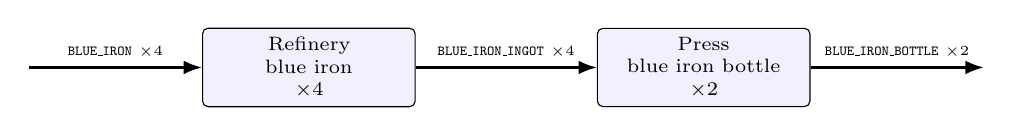
\begin{tikzpicture}[node distance=0.9cm and 2.3cm]
        \node[machinenode] (ref) {Refinery\\blue iron\\$\times 4$};
        \node[machinenode, right=of ref] (press) {Press\\blue iron bottle\\$\times 2$};
        \draw[prodarrow] ([xshift=-2.2cm]ref.west) -- node[edgelabel] {\texttt{BLUE\_IRON} $\times 4$} (ref.west);
        \draw[prodarrow] (ref.east) -- node[edgelabel] {\texttt{BLUE\_IRON\_INGOT} $\times 4$} (press.west);
        \draw[prodarrow] (press.east) -- node[edgelabel] {\texttt{BLUE\_IRON\_BOTTLE} $\times 2$} ([xshift=2.2cm]press.east);
    \end{tikzpicture}}
    \caption{Low difficulty production chain: 2 \texttt{BLUE\_IRON\_BOTTLE}.}
    \label{fig:chain-low}
\end{figure}
\vspace{0.9cm}

\begin{figure}[H]
    \centering
    \resizebox{\linewidth}{!}{
    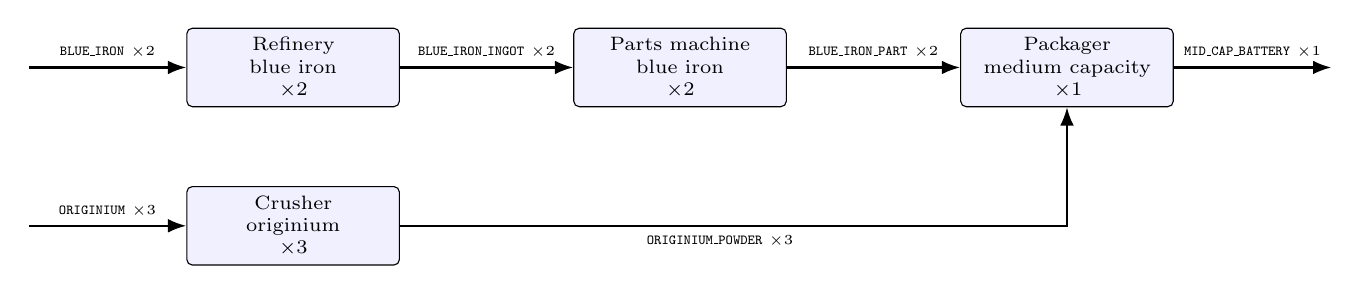
\begin{tikzpicture}[node distance=1.0cm and 2.2cm]
        \node[machinenode] (ref) {Refinery\\blue iron\\$\times 2$};
        \node[machinenode, right=of ref] (part) {Parts machine\\blue iron\\$\times 2$};
        \node[machinenode, right=of part] (pack) {Packager\\medium capacity\\$\times 1$};
        \node[machinenode, below=1.0cm of ref] (cru) {Crusher\\originium\\$\times 3$};

        \draw[prodarrow] ([xshift=-2.0cm]ref.west) -- node[edgelabel] {\texttt{BLUE\_IRON} $\times 2$} (ref.west);
        \draw[prodarrow] (ref.east) -- node[edgelabel] {\texttt{BLUE\_IRON\_INGOT} $\times 2$} (part.west);
        \draw[prodarrow] (part.east) -- node[edgelabel] {\texttt{BLUE\_IRON\_PART} $\times 2$} (pack.west);
        \draw[prodarrow] ([xshift=-2.0cm]cru.west) -- node[edgelabel] {\texttt{ORIGINIUM} $\times 3$} (cru.west);
        \draw[prodarrow] (cru.east) -| node[pos=0.24, fill=white, inner sep=1pt, below=2pt, font=\tiny] {\texttt{ORIGINIUM\_POWDER} $\times 3$} (pack.south);
        \draw[prodarrow] (pack.east) -- node[edgelabel] {\texttt{MID\_CAP\_BATTERY} $\times 1$} ([xshift=2.0cm]pack.east);
    \end{tikzpicture}}
    \caption{Medium difficulty production chain: 1 \texttt{MID\_CAP\_BATTERY}.}
    \label{fig:chain-medium}
\end{figure}
\vspace{0.9cm}

\begin{figure}[H]
    \centering
    \resizebox{\linewidth}{!}{
    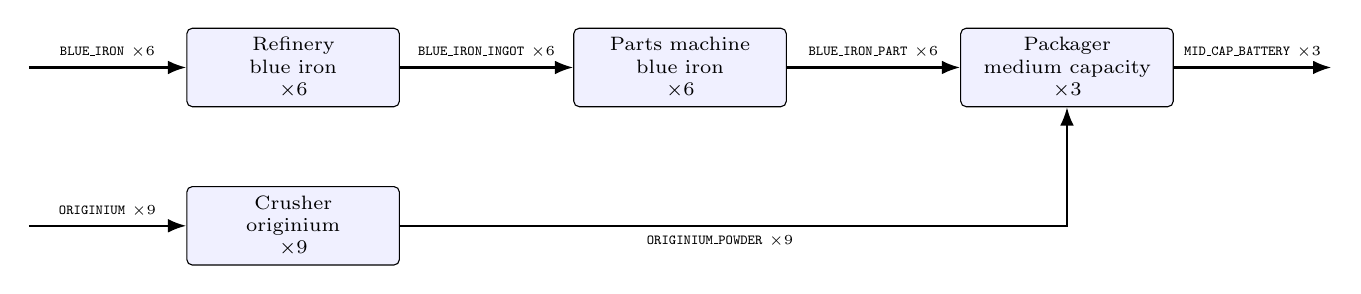
\begin{tikzpicture}[node distance=1.0cm and 2.2cm]
        \node[machinenode] (ref) {Refinery\\blue iron\\$\times 6$};
        \node[machinenode, right=of ref] (part) {Parts machine\\blue iron\\$\times 6$};
        \node[machinenode, right=of part] (pack) {Packager\\medium capacity\\$\times 3$};
        \node[machinenode, below=1.0cm of ref] (cru) {Crusher\\originium\\$\times 9$};

        \draw[prodarrow] ([xshift=-2.0cm]ref.west) -- node[edgelabel] {\texttt{BLUE\_IRON} $\times 6$} (ref.west);
        \draw[prodarrow] (ref.east) -- node[edgelabel] {\texttt{BLUE\_IRON\_INGOT} $\times 6$} (part.west);
        \draw[prodarrow] (part.east) -- node[edgelabel] {\texttt{BLUE\_IRON\_PART} $\times 6$} (pack.west);
        \draw[prodarrow] ([xshift=-2.0cm]cru.west) -- node[edgelabel] {\texttt{ORIGINIUM} $\times 9$} (cru.west);
        \draw[prodarrow] (cru.east) -| node[pos=0.24, fill=white, inner sep=1pt, below=2pt, font=\tiny] {\texttt{ORIGINIUM\_POWDER} $\times 9$} (pack.south);
        \draw[prodarrow] (pack.east) -- node[edgelabel] {\texttt{MID\_CAP\_BATTERY} $\times 3$} ([xshift=2.0cm]pack.east);
    \end{tikzpicture}}
    \caption{High difficulty production chain: 3 \texttt{MID\_CAP\_BATTERY}.}
    \label{fig:chain-high}
\end{figure}
\vspace{0.9cm}

\begin{figure}[H]
    \centering
    \resizebox{\linewidth}{!}{
    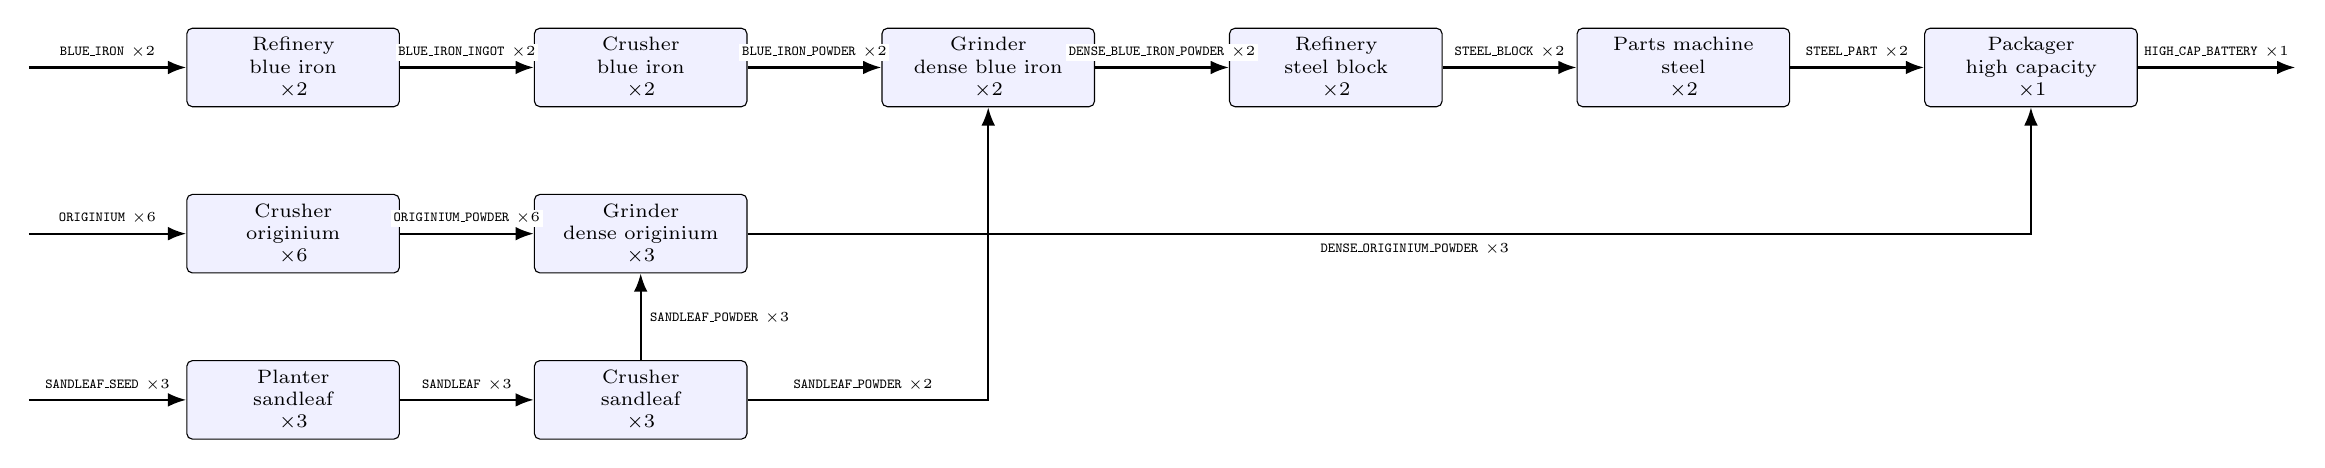
\begin{tikzpicture}[node distance=1.0cm and 1.7cm]
        \node[machinenode] (biref) {Refinery\\blue iron\\$\times 2$};
        \node[machinenode, right=of biref] (bicru) {Crusher\\blue iron\\$\times 2$};
        \node[machinenode, right=of bicru] (grindbi) {Grinder\\dense blue iron\\$\times 2$};
        \node[machinenode, right=of grindbi] (steelref) {Refinery\\steel block\\$\times 2$};
        \node[machinenode, right=of steelref] (steelpartm) {Parts machine\\steel\\$\times 2$};
        \node[machinenode, right=of steelpartm] (pack) {Packager\\high capacity\\$\times 1$};

        \node[machinenode, below=1.1cm of biref] (oricru) {Crusher\\originium\\$\times 6$};
        \node[machinenode, right=of oricru] (grindori) {Grinder\\dense originium\\$\times 3$};

        \node[machinenode, below=1.1cm of oricru] (plant) {Planter\\sandleaf\\$\times 3$};
        \node[machinenode, right=of plant] (leafcru) {Crusher\\sandleaf\\$\times 3$};

        \draw[prodarrow] ([xshift=-2.0cm]biref.west) -- node[edgelabel] {\texttt{BLUE\_IRON} $\times 2$} (biref.west);
        \draw[prodarrow] (biref.east) -- node[edgelabel] {\texttt{BLUE\_IRON\_INGOT} $\times 2$} (bicru.west);
        \draw[prodarrow] (bicru.east) -- node[edgelabel] {\texttt{BLUE\_IRON\_POWDER} $\times 2$} (grindbi.west);
        \draw[prodarrow] (grindbi.east) -- node[edgelabel] {\texttt{DENSE\_BLUE\_IRON\_POWDER} $\times 2$} (steelref.west);
        \draw[prodarrow] (steelref.east) -- node[edgelabel] {\texttt{STEEL\_BLOCK} $\times 2$} (steelpartm.west);
        \draw[prodarrow] (steelpartm.east) -- node[edgelabel] {\texttt{STEEL\_PART} $\times 2$} (pack.west);

        \draw[prodarrow] ([xshift=-2.0cm]oricru.west) -- node[edgelabel] {\texttt{ORIGINIUM} $\times 6$} (oricru.west);
        \draw[prodarrow] (oricru.east) -- node[edgelabel] {\texttt{ORIGINIUM\_POWDER} $\times 6$} (grindori.west);
        \draw[prodarrow] (grindori.east) -| node[pos=0.26, fill=white, inner sep=1pt, below=2pt, font=\tiny] {\texttt{DENSE\_ORIGINIUM\_POWDER} $\times 3$} (pack.south);

        \draw[prodarrow] ([xshift=-2.0cm]plant.west) -- node[edgelabel] {\texttt{SANDLEAF\_SEED} $\times 3$} (plant.west);
        \draw[prodarrow] (plant.east) -- node[edgelabel] {\texttt{SANDLEAF} $\times 3$} (leafcru.west);
        \draw[prodarrow] (leafcru.east) -| node[pos=0.24, fill=white, inner sep=1pt, above=2pt, font=\tiny] {\texttt{SANDLEAF\_POWDER} $\times 2$} (grindbi.south);
        \draw[prodarrow] (leafcru.north) -- node[pos=0.48, fill=white, inner sep=1pt, right=2pt, font=\tiny] {\texttt{SANDLEAF\_POWDER} $\times 3$} (grindori.south);

        \draw[prodarrow] (pack.east) -- node[edgelabel] {\texttt{HIGH\_CAP\_BATTERY} $\times 1$} ([xshift=2.0cm]pack.east);
    \end{tikzpicture}}
    \caption{Extreme difficulty production chain: 1 \texttt{HIGH\_CAP\_BATTERY}.}
    \label{fig:chain-extreme}
\end{figure}
\vspace{0.9cm}

\subsection{Metrics}

\begin{table}[H]
    \centering
    \caption{Evaluation metrics and calculation methods.}
    \label{tab:metrics}
    \begin{tabular}{L{0.26\linewidth} L{0.42\linewidth} L{0.22\linewidth}}
        \toprule
        Metric & Calculation method & Meaning \\
        \midrule
        Best Area & Minimum bounding-box area among valid or best available runs. & Spatial footprint. \\
        Best Belt Length & Minimum placed transport components among valid or best available runs. & Logistics length. \\
        Routing Success / 5 & Seeds where all material-flow edges connect. & Routability. \\
        Production Success / 5 & Seeds where the target amount is produced. & Production validity. \\
        \bottomrule
    \end{tabular}
\end{table}

\subsection{Procedure}

Each blueprint is evaluated with the same checks. Invalid or partially routed layouts are kept because failure rate matters. The report records best area, best belt length, routing success, production success, and qualitative examples.

\section{Results}
\label{sec:results}

\begin{table}[H]
    \centering
    \small
    \caption{Main benchmark results across three difficulty levels.}
    \label{tab:results}
    \setlength{\tabcolsep}{2pt}
    \begin{tabular}{@{}L{0.12\linewidth} L{0.18\linewidth} L{0.12\linewidth} L{0.12\linewidth} L{0.14\linewidth} L{0.18\linewidth}@{}}
        \toprule
        Difficulty & Family & Best Area $\downarrow$ & Best Belt Length $\downarrow$ & Routing Success / 5 $\uparrow$ & Production Success / 5 $\uparrow$ \\
        \midrule
        Low & Baseline & 312 & 32 & 100\% & 100\% \\
        Low & SA & 440 & 132 & 100\% & 100\% \\
        Low & FDP+SA & 140 & 27 & 100\%  & 100\% \\
        Low & SequenceSA & 170 & 48 & 100\%  & 100\%  \\
        Low & SequenceGA & 112 & 22 & 100\% & 100\% \\
        Low & Flow/CP & 120 & 27 & 100\% & 100\% \\
        \addlinespace
        Medium & Baseline & 621 & 104 & 100\% & 100\% \\
        Medium & SA & 285 & 49 & 100\% & 100\% \\
        Medium & FDP+SA & 272 & 66 & 100\% & 100\% \\
        Medium & SequenceSA & 165 & 46 & 100\%  & 100\%  \\
        Medium & SequenceGA & 165 & 45 & 100\%  & 100\% \\
        Medium & Flow/CP & 208 & 66 & 100\% & 100\% \\
        \addlinespace
        High & Baseline & FAIL & FAIL & 0\% & 0\% \\
        High & SA & FAIL & FAIL & 0\% & 0\% \\
        High & FDP+SA & FAIL & FAIL & 0\% & 0\% \\
        High & SequenceSA & 816 & 241 & 100\% & 100\% \\
        High & SequenceGA & 585 & 161 & 100\% & 100\% \\
        High & Flow/CP & 1269 & 310 & 100\% & 100\% \\
        \bottomrule
    \end{tabular}
\end{table}

\begin{table}[H]
    \centering
    \caption{SequenceGA extreme test.}
    \label{tab:sequencega-extreme}
    \setlength{\tabcolsep}{2pt}
    \begin{tabular}{@{}L{0.09\linewidth} L{0.15\linewidth} L{0.21\linewidth} L{0.23\linewidth} L{0.26\linewidth}@{}}
        \toprule
        Test & Best Area $\downarrow$ & Best Belt Length $\downarrow$ & Routing Success / 5 $\uparrow$ & Production Success / 5 $\uparrow$ \\
        \midrule
        Extreme & 3069 & 539 & 100\% & 100\% \\
        \bottomrule
    \end{tabular}
\end{table}

\subsection{Best Blueprint Examples}

The examples show best generated blueprints. SequenceGA also includes an in-game screenshot. A compact legend precedes the ASCII renders.

\begin{table}[H]
    \centering
    \caption{Legend for simulated blueprint examples.}
    \label{tab:blueprint-legend}
    \begin{tabular}{L{0.20\linewidth} L{0.64\linewidth}}
        \toprule
        Symbol & Meaning \\
        \midrule
        \texttt{REF} & Refinery. \\
        \texttt{CRU} & Crusher. \\
        \texttt{PRT} & Parts machine. \\
        \texttt{PRS} & Press. \\
        \texttt{PAK} & Packager. \\
        \texttt{GRD} & Grinder. \\
        \texttt{PLT} / \texttt{EXT} & Planter / extractor. \\
        \texttt{.} & Empty cell. \\
        \texttt{>} \texttt{<} \texttt{\textasciicircum} \texttt{v} & Belt direction. \\
        Corner belt cell & Belt turn. \\
        \texttt{[X]} & Crosser. \\
        \texttt{[S]} & Splitter/router. \\
        \texttt{[M]} & Merger. \\
        \texttt{X01}, \texttt{S01}, or direction plus number & Component currently carrying one item. \\
        \bottomrule
    \end{tabular}
\end{table}

\begin{figure}[H]
    \centering
    \blueprintimage{FDP_SA_Medium.png}
    \caption{Example Result: FDP\_SA simulated blueprint on medium difficulty.}
    \label{fig:example-fdp-sa-medium}
\end{figure}

\begin{figure}[H]
    \centering
    \blueprintimage{SequenceSA_High.png}
    \caption{Eample Result: SequeceSA simulated blueprint on high difficulty.}
    \label{fig:example-sequence-sa-high}
\end{figure}

\begin{figure}[H]
    \centering
    \blueprintimage{SequenceGA_High.png}
    \caption{Example Result: SequenceGA simulated blueprint on high difficulty.}
    \label{fig:example-sequence-ga-high}
\end{figure}

\begin{figure}[H]
    \centering
    \blueprintimage{Actual_High.png}
    \caption{Real Blueprint in Game: SequenceGA simulated blueprint on high difficulty.}
    \label{fig:example-actual-high}
\end{figure}

\begin{figure}[H]
    \centering
    \blueprintimage{SequenceGA_High_working.png}
    \caption{Working Status: SequenceGA simulating blueprint on high difficulty.}
    \label{fig:example-sequence-ga-working}
\end{figure}


\section{Discussion}
\label{sec:discussion}

The results show that AutoBlueprint is not only a placement problem, but a joint reasoning problem over recipes, ports, routing, and simulation. A compact rectangle is useful only when the belts can still be routed and the simulated factory can produce the requested amount. This explains why the best agents are not the ones with the simplest area objective, but the ones that combine production graph structure with routing feedback.

\subsection{Answer to the Research Question}

The research question asks whether autonomous agents can generate compact, routable, and productive System B blueprints. The answer is positive, but only when symbolic production reasoning is coupled with routing-aware spatial search. The deterministic baseline works on easier chains but fails on high difficulty, while SA and FDP+SA improve flexibility without fully solving dense multi-input routing.

Sequence-based agents perform better because they search over production cells rather than isolated coordinates. SequenceSA reaches a valid high-difficulty result, and SequenceGA gives the strongest result in the table: best area 585 and best belt length 161, with full routing and production success. Its fan in cell rule keeps one to one suppliers near their consumers, reducing both edge placement and belt length. Thus, the best performance comes from combining optimisation with blueprint-specific structure.

\subsection{Strengths}

The strongest engineering feature is the extensible environment model. The \texttt{grid\_map}, \texttt{registry}, material catalogue, recipe catalogue, building model, and transport components are separated cleanly, so changed products or new buildings, materials, and recipes require local catalogue updates rather than agent rewrites.

The environment also contains transport logic and tick-based simulation for belts, ports, crossers, generated inputs and outputs, inventories, and production ticks. A generated blueprint can therefore be tested as a working material-flow system, making evaluation closer to the real game environment than a purely geometric check.

The agent design is also broad: rule-based placement, simulated annealing, force-directed placement, sequence-pair search, B* tree packing, genetic search, negotiated routing, and min cost flow assignment are compared in one framework. This shows a progression from simple heuristics to hybrid agents, especially in SequenceGA, where evolutionary search is built on meaningful production cells.

\subsection{Limitations}

Result quality depends strongly on the target product. A layout rule that works well for one chain may be poor for another with different fan in, fan out, port pressure, or raw input demand. This makes it difficult to build one evaluation system that is fair for all products; area, belt length, routing success, and production success are useful but do not always agree.

Computational cost is another limitation. More detailed agents spend more time on routing trials, repair, rotation search, and simulation. As building count grows, the combinations of positions, orientations, ports, and routes grow rapidly, so high-difficulty tasks are hard to solve with a single pure algorithm.

Finally, the environment is still an abstraction. It captures the main System B constraints used here, but not every game mechanic or export format.

\subsection{Finding}

A key finding is that SA and GA parameter tuning alone gives limited improvement once the search is stable. Larger gains came from adding domain knowledge, such as SequenceGA's fan in cell rule, which encodes the observation that a one to one supplier should usually be near its consumer. Effective agents therefore need both general search and blueprint-specific construction rules.

\section{Conclusion and Future Work}
\label{sec:conclusion}

\subsection{Conclusion}

AutoBlueprint demonstrates that factory blueprint generation can be formulated as an autonomous intelligent agent problem. It builds an extensible System B environment with catalogues, building models, transport components, and tick-based simulation, so agent outputs can be checked as working production systems rather than only static layouts.

The experiments show that compact, routable, and productive blueprints can be generated when production planning, placement search, routing, and simulation are linked. SequenceGA gives the strongest high-difficulty result because it combines genetic search with production-cell structure and the fan in rule. Overall, the project shows that hybrid methods are most suitable: optimisation explores alternatives, while domain knowledge gives the search a useful structure.

\subsection{Future Work}

The main future direction follows from the finding that experience-based blueprint rules can matter more than parameter tuning. Good rules improve initial layouts and reduce computation by avoiding poor search regions. This suggests that reinforcement learning could perform well, because an agent could learn reusable placement and routing policies from repeated blueprint attempts \cite{sutton2018reinforcement}. It was not completed here because the required training time, memory, and computation exceeded the project limits.

Future work will add more blueprint-specific rules, including common subchain grouping, input and output corridor selection, fan in and fan out placement, and crosser usage. Another extension is to complete the game's building and product catalogue, allowing wider and more realistic benchmarks.

A more authoritative evaluation scheme is also needed. A full benchmark should consider more products, map shapes, game-specific constraints, and a clearer balance between area, belt length, production rate, routing complexity, and robustness. Finally, System A could be completed to compare the Mindustry-style logistics model with System B and study how transport rules change planning difficulty.

\section*{AI Statement}

AI tools were used to assist with report structure planning and minor language refinement. All components were first written by author and were further checked after AI modified.

\bibliographystyle{plain}
\bibliography{references}

\end{document}
